\documentclass[11pt, english, fleqn, DIV=15, headinclude, BCOR=1cm]{scrartcl}

\usepackage[
    bibatend,
    color,
]{../header}

\usepackage{booktabs}
\usepackage{pdflscape}

\usepackage{tikz}

\usepackage[tikz]{mdframed}
\newmdtheoremenv[%
    backgroundcolor=black!5,
    innertopmargin=\topskip,
    splittopskip=\topskip,
]{theorem}{Theorem}[section]

\newmdenv[%
    backgroundcolor=black!5,
    frametitlebackgroundcolor=black!10,
    roundcorner=5pt,
    skipabove=\topskip,
    innertopmargin=\topskip,
    splittopskip=\topskip,
    frametitle={Problem statement},
    frametitlerule=true,
]{problem}

\newmdenv[%
    backgroundcolor=white,
    frametitlebackgroundcolor=black!10,
    roundcorner=5pt,
    skipabove=\topskip,
    innertopmargin=\topskip,
    innerbottommargin=8cm,
    splittopskip=\topskip,
    frametitle={Side question},
    frametitlerule=true,
    %nobreak=true,
]{question}


\hypersetup{
    pdftitle=
}

\newcommand\inv{^{-1}}

\newcounter{totalpoints}
\newcommand\punkte[1]{#1\addtocounter{totalpoints}{#1}}

\newcounter{problemset}
\setcounter{problemset}{5}

\subject{physics751 -- Group Theory}
\ihead{physics751 -- Problem Set \arabic{problemset}}

\title{Problem Set \arabic{problemset}}

\publishers{Group 1 -- Patrick Matuschek}
\ofoot{Group 1 -- Patrick Matuschek}

\author{
    Martin Ueding \\ \small{\href{mailto:mu@martin-ueding.de}{mu@martin-ueding.de}}
}
\ifoot{Martin Ueding}

\ohead{\rightmark}

\begin{document}

\maketitle

\section{A representation on homogeneous functions}

\newcommand\Ra{\tens R^{(\text a)}}
\newcommand\Rb{\tens R^{(\text b)}}

There are two spaces here, $\R^2$ and $\R^3$. The problem set says that $\R^2$
is invariant to two given transformations from $O(2)$. I believe that we are
just given two elements from $O(2)$ here such that those elements are the
generators of a subgroup which then happens to be discrete. Then we avoid
working with a continuous group which we had not covered in class yet.

Regarding this invariance, I am not sure about the actual meaning. When I take
a vector $\vec r$ from $\R^2$ and apply the matrix $\Ra$ or $\Rb$ to it, it
will become a different vector. What stays invariant is $\bracket{\vec r, \vec
r}$, which would also left invariant by any member of $O(2)$. So “the space is
invariant under” probably means that the set $\{ \vec r \colon \vec r \in
\R^2\} = \R^2$ (which is just $\R^2$) is the same as $\{ \Ra \vec r \colon \vec
r \in \R^2\}$? Such that I can do a parametric plot of the space, it will stay
just the same?

Now there is a map $\phi: \R^2 \mapsto \R^3$ defined as the following:
\[
    \begin{pmatrix}
        x \\ y
    \end{pmatrix}
    \to
    \begin{pmatrix}
        x^2 \\ xy \\ y^2
    \end{pmatrix}.
\]
Figure~\ref{fig:3d} shows the parametric plot
\[
    \{ \vec \phi(\tens X \vec r) \colon \vec r \in [-2,2]^2 \subset \R^2 \}
\]
where $\tens X$ is the identity, $\Ra$ and $\Rb$, each in a different color.
The spaces that are spanned like this are all the same, although the individual
points from $\R^2$ are not mapped to the same points in the image of $\phi$.

\begin{figure}[htbp]
    \centering
    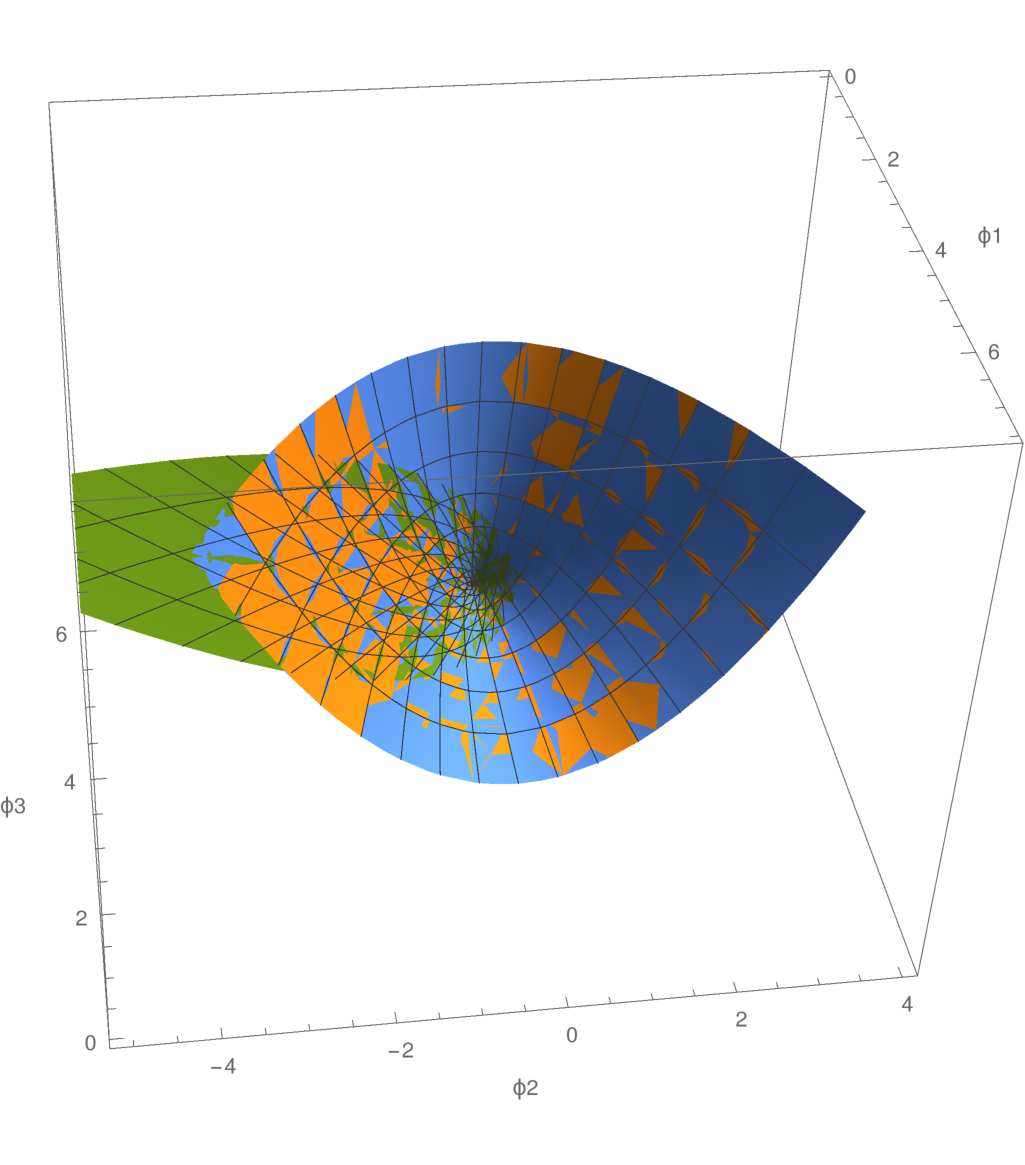
\includegraphics[width=.6\linewidth]{phi.pdf}
    \caption{%
        A parametric plot of $\vec\phi(\vec r)$, $\vec\phi(\Ra \vec r)$ and
        $\vec\phi(\Rb \vec r)$. $\vec r$ is taken are taken from $[-2,2]^2
        \subset \R^2$. The coloring glitches show that the three surfaces lie
        within each other, so the surfaces that are created for all $\vec r$
        are equal.
    }
    \label{fig:3d}
\end{figure}

I believe that the following equation must hold because of the representation
axiom $\tens D(gh) = \tens D(g) \tens D(h)$:
\[
    \vec \phi(\tens R \vec r) = \tens D(\tens R) \vec \phi(\vec r).
\]
Applying the group element $R \in O(2)$, represented by its matrix $\tens R$
before the application of $\phi$ must yield the same result as postmultiplying
with the $\R^3$ representation of $R$.

\subsection{Part (a)}

So I apply this idea to $\Ra$:
\[
    \vec\phi(\Ra \vec r)
    =
    \vec\phi\del{
        \begin{pmatrix}
            x \\ -y
        \end{pmatrix}
    }
    = 
    \begin{pmatrix}
        x^2 \\ -xy \\ y^2
    \end{pmatrix}
    =
    \begin{pmatrix}
        1 & 0 & 0 \\
        0 & -1 & 0 \\
        0 & 0 & 1
    \end{pmatrix}
    \begin{pmatrix}
        x^2 \\ xy \\ y^2
    \end{pmatrix}.
\]
Therefore, I say that
\[
    \tens D(\Ra) = 
    \begin{pmatrix}
        1 & 0 & 0 \\
        0 & -1 & 0 \\
        0 & 0 & 1
    \end{pmatrix}.
\]

\subsection{Part (b)}

This works similarly for $\Rb$ as well, just a bit more calculations:
\[
    \vec \phi(\Rb \vec r)
    =
    \vec \phi\del{
        \frac12
        \begin{pmatrix}
            -x + \sqrt3 y \\
            \sqrt3 x - y
        \end{pmatrix}
    }
    =
    \frac14
    \begin{pmatrix}
        x^2 - 2\sqrt3 xy + 3y^2 \\
        - \sqrt3 x^2 - 2 xy + \sqrt3 y^2 \\
        e x^2 - 2 \sqrt 3 xy y^2
    \end{pmatrix}
    =
    \frac14
    \begin{pmatrix}
        1 & -2\sqrt3 & 3 \\
        -\sqrt3 & -2 & \sqrt3 \\
        3 & -2\sqrt3 & 1
    \end{pmatrix}
    \begin{pmatrix}
        x^2 \\ xy \\ y^2
    \end{pmatrix}.
\]
Then
\[
    \tens D(\Rb) =
    \begin{pmatrix}
        1 & -2\sqrt3 & 3 \\
        -\sqrt3 & -2 & \sqrt3 \\
        3 & -2\sqrt3 & 1
    \end{pmatrix}.
\]



\end{document}

% vim: spell spelllang=en tw=79
